\chapter{胺与含氮化合物}\label{ch:b2:amines}

不再新鲜的鱼会散发三甲胺的气味，三甲胺是一种小分子挥发性胺。
挤几滴柠檬汁即可除去这股气味：酸使胺质子化，
生成的铵离子带电，无法挥发。氮原子上的孤对电子使胺呈碱性、具有亲核性；
与羰基相连时则生成\omterm{def:b2:amines:imine}{亚胺}，
蛋白质借此完成其化学功能，化学家也借此制备胺；在芳环上，
经重氮盐可开辟通往偶氮染料的道路，
这些染料曾使十九世纪五彩斑斓。

\begin{recall}
本科一年级分册：布朗斯特酸和碱，$\mathrm pK_a$ 与优势区域图，
亲核试剂与双分子取代，半缩醛和缩醛，氢负离子供体，
有机镁试剂，碳原子的类别。\Cref{ch:b2:aromatic-substitution}：
硝化，硝基\omterm{def:b2:aromatic-substitution:arene}{芳烃}的还原。第 1 册：胺和酰胺。
\end{recall}

\begin{omfigure}
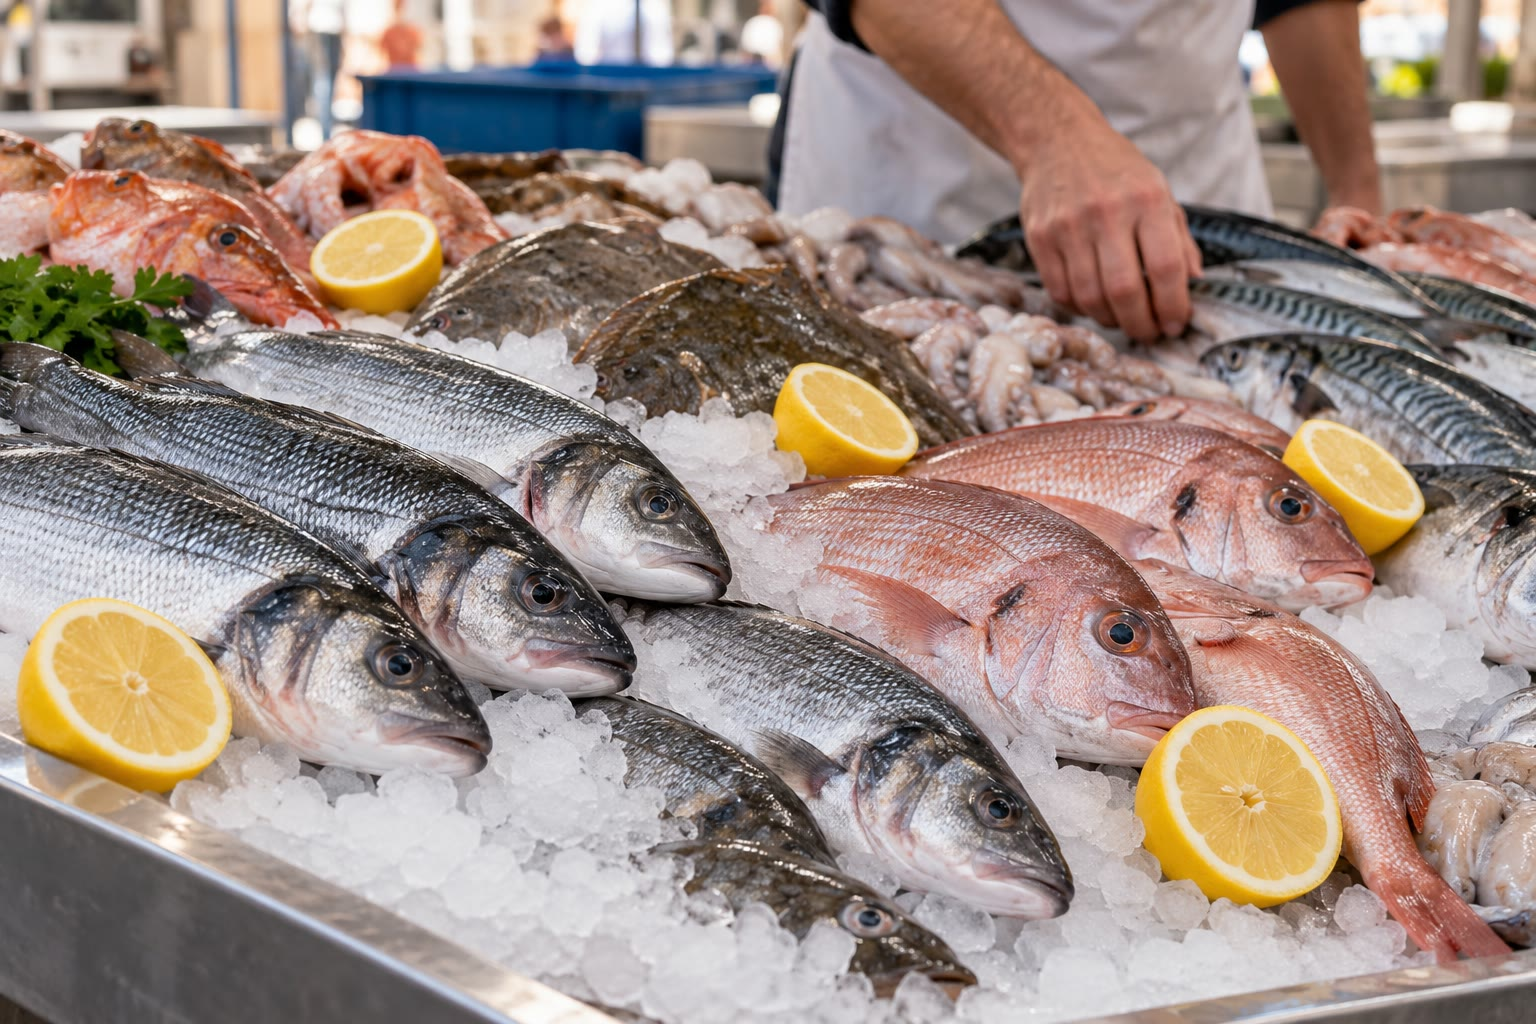
\includegraphics[width=0.6\linewidth]{images/book3/ai/b2-23-fish-stall.jpg}

{\small 鱼摊：柠檬切成两半，摆放在鱼之间。柠檬的酸使
鱼中的三甲胺转化为不挥发的铵离子。}
\end{omfigure}

\section{结构与碱性}

\begin{definition}[胺的分类]\label{def:b2:amines:class}
按与氮相连的碳基数目，胺分为\emph{伯胺}\index{伯胺} \ce{RNH2}、\emph{仲胺}
\index{仲胺} \ce{R2NH}和\emph{叔胺}\index{叔胺}
\ce{R3N}三类。\emph{季铵
离子}\index{季铵离子} \ce{R4N+}含四个碳基，不含孤对电子。
\end{definition}

胺中的氮原子大致呈四面体构型，孤对电子占据
第四个位置。三个基团各不相同的\omterm{def:b2:amines:class}{叔胺}原则上具有手性，但无法
拆分：分子经平面构型翻转，好比风中翻转的雨伞，
在室温下每秒翻转约十亿次。

\begin{proposition}[碱性]\label{prop:b2:amines:basicity}
在水中，烷基胺的碱性强于氨（其铵离子的 $\mathrm pK_a$
约为 10 至 11，氨为 9.26），芳胺弱得多（苯胺正离子为 4.60），酰胺
几乎没有碱性（质子化的乙酰胺约为 $-0.6$）。
\end{proposition}

\begin{proof}[论证]
烷基将电子云推向氮原子（诱导效应），并稳定
铵离子的正电荷。在水中，氢键引起的溶剂化同样重要：
含 \ce{N-H} 键越多的离子溶剂化越好，这也是三甲铵（9.80）
的酸性弱于铵，却强于二甲铵（10.73）。在苯胺中，孤对电子
离域到芳环上，质子化时即失去；在酰胺中则离域到
羰基氧上，质子化较弱地发生在氧原子上。
% ledger: kb:NH3, pka:methylammonium, pka:dimethylammonium, pka:trimethylammonium, pka:anilinium, pka:ethanamideH
\end{proof}

\begin{omfigure}
\begin{tikzpicture}[font=\small, x=0.85cm]
  \draw[->, thick] (-1.5,0) -- (11.8,0) node[below right] {$\mathrm pK_a$};
  \foreach \x in {0,2,4,6,8,10} \draw (\x,0.1) -- (\x,-0.1) node[below, font=\scriptsize] {\x};
  \foreach \x/\l in {-0.6/{\ce{CH3CONH3+}}, 4.60/{\ce{C6H5NH3+}}} {
    \draw[omDef, thick] (\x,0) -- (\x,0.5);
    \node[font=\scriptsize, anchor=south] at (\x,0.5) {\l};
  }
  \foreach \x/\l/\y/\h in {9.26/{\ce{NH4+} (9.26)}/1.95/1.2, 9.80/{\ce{(CH3)3NH+} (9.80)}/1.45/0.85, 10.66/{\ce{CH3NH3+} (10.66)}/0.95/0.5, 10.73/{\ce{(CH3)2NH2+} (10.73)}/0.45/0.25} {
    \draw[omDef, thick] (\x,0) -- (\x,\h);
    \draw[black!40] (\x,\h) -- (12.2,\y);
    \node[font=\scriptsize, anchor=west] at (12.2,\y) {\l};
  }
  \node[font=\scriptsize, anchor=north west] at (-1.4,-0.5) {弱碱};
  \node[font=\scriptsize, anchor=north east] at (11.7,-0.5) {强碱};
\end{tikzpicture}

{\small 若干含氮碱的共轭酸的 $\mathrm pK_a$，在
\qty{25}{\degreeCelsius} 下测得：该值越高，碱性越强。}
% ledger: kb:NH3, pka:methylammonium, pka:dimethylammonium, pka:trimethylammonium, pka:anilinium, pka:ethanamideH
\end{omfigure}

\section{胺作为亲核试剂}

胺通过双分子取代进攻卤代烷。产物是取代程度更高的胺，
其亲核性至少与原来的胺相当，并与卤代烷竞争：
氨的烷基化会得到\omterm{def:b2:amines:class}{伯胺}、\omterm{def:b2:amines:class}{仲胺}和\omterm{def:b2:amines:class}{叔胺}的混合物，以及
季铵盐。

\begin{proposition}[多烷基化]\label{prop:b2:amines:polyalkylation}
氨或\omterm{def:b2:amines:class}{伯胺}的直接烷基化得到混合物；只有彻底烷基化
为季铵盐时，产物才纯净。
\end{proposition}

\begin{proof}[论证]
每次烷基化都在氮上留下一对孤对电子，而新烷基使该氮的电子云更加丰富，
产物与剩余卤代烷以相近速率反应。只有当
氮上不再有孤对电子、即形成 \ce{R4N+} 时，反应才停止。
\end{proof}

不含过度烷基化产物的\omterm{def:b2:amines:class}{伯胺}需间接制备：一是加布里埃尔合成法
（对邻苯二甲酰\omterm{def:b2:amines:imine}{亚胺}的氮原子进行烷基化，该氮上仅带一个酸性氢，随后
释放出胺），二是腈、酰胺或硝基化合物的还原，或
经\omterm{def:b2:amines:reductive-amination}{还原胺化}（见下文）。

\section{亚胺与烯胺}

\begin{definition}[亲核加成]\label{def:b2:amines:nucleophilic-addition}
对羰基的\emph{亲核加成}\index{亲核加成}是指亲核试剂
进攻羰基碳原子，使其变为四面体构型，\ce{C=O} 中的 $\pi$ 键
变为氧原子上的孤对电子。
\end{definition}

\begin{definition}[半缩胺、亚胺与烯胺]\label{def:b2:amines:imine}
\omterm{def:b2:amines:class}{伯胺}与醛或酮加成，得到\emph{半缩胺}\index{半缩胺}
（连有 \ce{OH} 和 \ce{NHR} 的碳原子）；其脱水得到\emph{亚胺}\index{亚胺}
$\mathrm{R_2C{=}NR'}$。\omterm{def:b2:amines:class}{仲胺}不能形成中性亚胺，脱水后得到
\emph{烯胺}\index{烯胺} $\mathrm{R_2C{=}CR{-}NR'_2}$，双键转移至相邻的碳原子上。
\end{definition}

\begin{omfigure}
\setchemfig{atom sep=1.9em}
\schemestart
\chemfig{R_2C=O} \+ \chemfig{H_2N-R'}
\arrow{<=>}
\chemfig{R_2C(-[2]OH)-NH-R'}
\arrow{<=>[\ce{H+}][$-$ \ce{H2O}]}
\chemfig{R_2C=N-R'}
\schemestop
\par\vspace{6pt}

{\small \omterm{def:b2:amines:imine}{亚胺}的生成：胺对羰基的\omterm{def:b2:amines:nucleophilic-addition}{亲核加成}得到
\omterm{def:b2:amines:imine}{半缩胺}；酸催化使其 \ce{OH} 变为离去基团（\ce{-OH2+}），水离去，
氮原子上的孤对电子形成 \ce{C=N} 双键。每一步均可逆：过量的水
使\omterm{def:b2:amines:imine}{亚胺}水解回羰基化合物和胺。}
\end{omfigure}

\begin{proposition}[pH 最适值]\label{prop:b2:amines:imine-ph}
\omterm{def:b2:amines:imine}{亚胺}在弱酸性溶液中生成最快，pH 约为 4 至 5。
\end{proposition}

\begin{proof}[论证]
第一步需要游离的胺（其孤对电子）参与；酸性过强时胺被
质子化（$\mathrm pK_a$ 约为 10），使亲核试剂失效。脱水需要酸使
羟基质子化；pH 高时脱水很慢。反应速率即两种需求的乘积，
在两者之间最大。
\end{proof}

\begin{definition}[还原胺化]\label{def:b2:amines:reductive-amination}
\emph{还原胺化}\index{还原胺化}是指将羰基化合物与
胺，通过生成\omterm{def:b2:amines:imine}{亚胺}（或\omterm{def:b2:amines:imine}{亚胺}离子）并在同一反应体系中将其还原，
转化为取代程度更高的胺，通常使用氰基\omterm{def:b2:alkene-redox:hydroboration}{硼氢化}钠 \ce{NaBH3CN}。
\end{definition}

\begin{proposition}[还原胺化的选择性]\label{prop:b2:amines:reductive-amination}
pH 约为 6 时，\ce{NaBH3CN} 还原\omterm{def:b2:amines:imine}{亚胺}离子的速度远快于还原羰基化合物，
因此可得到胺，而醛或酮不会被还原为醇。
\end{proposition}

\begin{proof}[论证]
氰基使 \ce{BH3CN-} 成为较弱的氢负离子供体，对中性羰基而言太弱，但
足以还原质子化的带正电的\omterm{def:b2:amines:imine}{亚胺}离子，后者是更好的亲电试剂。
\end{proof}

\section{重氮盐}

\begin{definition}[重氮化学]\label{def:b2:amines:diazonium}
\emph{重氮离子}\index{重氮离子}是一种阳离子 \ce{R-N+#N}。\emph{重氮化}\index{重氮化}
是指在亚硝酸钠与强酸作用下，于
0--\qty{5}{\degreeCelsius}，将伯芳胺转化为芳基重氮盐。在\emph{桑德迈尔反应}\index{桑德迈尔反应}中，一种亚铜盐
（\ce{CuCl}、\ce{CuBr}、\ce{CuCN}）将重氮基以 Cl、Br 或 CN 取代，同时
放出氮气。在\emph{偶氮偶联}\index{偶氮偶联}中，重氮离子作为较弱的亲电试剂，
进攻活化的芳环，生成偶氮化合物 $\mathrm{Ar{-}N{=}N{-}Ar'}$。
\end{definition}

\begin{proposition}[重氮离子的稳定性]\label{prop:b2:amines:diazonium}
芳基重氮盐可在低温水溶液中保存并使用；烷基\omterm{def:b2:amines:diazonium}{重氮离子}
立即失去氮气。
\end{proposition}

\begin{proof}[论证]
氮气是极好的离去基团（它是非常稳定的分子，离去时熵增较大）。对于
烷基，失去 \ce{N2} 后留下碳正离子，或直接被水进攻，该离子
不能稳定存在。芳基正离子非常不稳定（环平面内有一空的 $\sigma$ 轨道，
未被 $\pi$ 体系稳定），而芳基\omterm{def:b2:amines:diazonium}{重氮离子}的 \ce{C-N} 键因与环共轭而增强：
低温下它可以存在；加热后分解，
水以 \ce{OH} 取代重氮基。
\end{proof}

\begin{omfigure}
\begin{tikzpicture}[font=\small, >={Stealth}]
  \node[cyclenode] (d) at (0,0) {\ce{Ar-N2+}};
  \foreach \a/\t/\c in {90/{\ce{Ar-Cl}}/{\ce{CuCl}}, 150/{\ce{Ar-Br}}/{\ce{CuBr}}, 210/{\ce{Ar-CN}}/{\ce{CuCN}},
                        270/{\ce{Ar-OH}}/{\ce{H2O}，温热}, 330/{\ce{Ar-H}}/{\ce{H3PO2}}, 30/{$\mathrm{Ar{-}N{=}N{-}Ar'}$}/{活化的 \ce{ArH}}} {
    \node[cyclenode] (p\a) at (\a:2.6) {\t};
    \draw[->, thick] (d) -- (p\a) node[midway, font=\scriptsize, fill=white, inner sep=1pt] {\c};
  }
\end{tikzpicture}

{\small 芳基重氮盐的反应。\ce{N2+} 基团可被卤素或
氰基取代（\omterm{def:b2:amines:diazonium}{桑德迈尔反应}，亚铜盐），被 \ce{OH}（温水）取代，或被 H（次磷酸）取代，或
保留下来进行\omterm{def:b2:amines:diazonium}{偶氮偶联}。}
\end{omfigure}

\begin{method}[经重氮盐的合成路线]\label{met:b2:amines:diazonium-routes}
\begin{enumerate}
  \item 利用氨基（强\omterm{def:b2:aromatic-substitution:directing}{邻/对位定位基}）引入其他基团，然后
        经重氮盐将其转化。
  \item 以 H 取代它，以得到直接取代无法获得的
        取代模式（由苯胺制得 1,3,5-三溴苯）。
  \item 以 CN 取代它，再水解为羧酸：在环上引入 \ce{-COOH} 的一种方法。
\end{enumerate}
\end{method}

\begin{method}[胺的制备]\label{met:b2:amines:make-amine}
\begin{enumerate}
  \item 烷基链上的\omterm{def:b2:amines:class}{伯胺}：盖布瑞尔合成法，或还原腈（碳原子数
        比制备腈所用的卤代烷多一个），或还原酰胺。
  \item \omterm{def:b2:amines:class}{仲胺}或\omterm{def:b2:amines:class}{叔胺}：用合适的羰基化合物与
        合适的胺进行\omterm{def:b2:amines:reductive-amination}{还原胺化}。
  \item 芳胺：先硝化，再还原（用铁或锡加酸，或
        \omterm{def:b2:alkene-redox:hydrogenation}{催化氢化}）。
\end{enumerate}
\end{method}

\section{腈}

\begin{definition}[腈]\label{def:b2:amines:nitrile}
\emph{腈}\index{腈}是一种化合物 \ce{R-C#N}，可由卤代烷
与氰根离子发生取代，或经\omterm{def:b2:amines:diazonium}{桑德迈尔反应}制得。
\end{definition}

\begin{proposition}[腈的反应]\label{prop:b2:amines:nitrile}
腈在酸性或碱性条件下水解，先生成酰胺，再生成羧酸；它
可被氢化铝锂还原为\omterm{def:b2:amines:class}{伯胺} \ce{RCH2NH2}；有机镁试剂
对其加成一次，生成的\omterm{def:b2:amines:imine}{亚胺}经水解得到酮。
\end{proposition}

\begin{proof}[论证]
腈碳与羰基碳一样具有亲电性：水（经酸活化，或以
氢氧根形式）加成到其上，经互变异构后得到酰胺，其水解在
\cref{ch:b2:acyl-substitution}中讨论。氢负离子加成两次。有机镁试剂加成一次，
生成不再反应的\omterm{def:b2:amines:imine}{亚胺}负离子；随后水将\omterm{def:b2:amines:imine}{亚胺}水解为酮。
\end{proof}

\begin{safety}{\ghs[5mm]{GHS03}\,\ghs[5mm]{GHS06}\,\ghs[5mm]{GHS08}\,\ghs[5mm]{GHS09}}
苯胺和 \textit{N},\textit{N}-二甲基苯胺经皮肤接触有毒；亚硝酸钠
有毒且具有氧化性；氰基\omterm{def:b2:alkene-redox:hydroboration}{硼氢化}钠遇酸会释放氰化氢，须在
通风橱中使用。干燥的重氮盐可能爆炸：应始终保持低温、置于溶液中，并
随即使用。
% ledger: ghs:aniline, ghs:dimethylaniline, ghs:NaNO2, ghs:NaBH3CN, ghs:sulfanilic-acid
\end{safety}

\section{练习}

\begin{exercise}[$\star$]\label{exo:b2:amines:1}
给出下列物质的类别：丙-1-胺、\textit{N}-甲基乙胺、三乙胺、
氯化四甲铵、苯胺。
\end{exercise}

\begin{exercise}[$\star$]\label{exo:b2:amines:2}
按碱性从弱到强排序：氨、甲胺、苯胺、乙酰胺。
\end{exercise}

\begin{exercise}[$\star$]\label{exo:b2:amines:3}
写出由环己酮与甲胺生成的\omterm{def:b2:amines:imine}{亚胺}及反应条件。
\end{exercise}

\begin{exercise}[$\star$]\label{exo:b2:amines:4}
以氯化重氮苯为原料，写出其与 \ce{CuBr}、\ce{CuCN}、温水
以及与碱性苯酚作用的产物。
\end{exercise}

\begin{exercise}[$\star\star$]\label{exo:b2:amines:5}
pH 为 7 时三甲胺以哪种形式为主？比例为多少？解释柠檬汁的作用，以及
如何将胺从有机溶剂萃取到水中。
\end{exercise}

\begin{exercise}[$\star\star$]\label{exo:b2:amines:6}
写出环己酮与吡咯烷生成的\omterm{def:b2:amines:imine}{烯胺}，并解释为何\omterm{def:b2:amines:class}{仲胺}
不能生成\omterm{def:b2:amines:imine}{亚胺}。
\end{exercise}

\begin{exercise}[$\star\star$]\label{exo:b2:amines:7}
用\omterm{def:b2:amines:reductive-amination}{还原胺化}法制备 \textit{N}-苄基丙-2-胺 \ce{C6H5CH2NHCH(CH3)2}，给出两组
可行的试剂组合。
\end{exercise}

\begin{exercise}[$\star\star$]\label{exo:b2:amines:8}
苯甲腈与溴化乙基镁反应，随后与酸的水溶液作用。写出产物。
\end{exercise}

\begin{exercise}[$\star\star$]\label{exo:b2:amines:9}
写出己-1-胺的盖布瑞尔合成，并解释为何不生成\omterm{def:b2:amines:class}{仲胺}。
\end{exercise}

\begin{exercise}[$\star\star\star$]\label{exo:b2:amines:10}
以苯胺为原料制备 1,3,5-三溴苯。
\end{exercise}

\begin{exercise}[$\star\star\star$]\label{exo:b2:amines:11}
以 4-硝基苯胺和苯酚为原料设计一种偶氮染料：写出\omterm{def:b2:amines:diazonium}{重氮化}、
偶联（位置与 pH）及产物。
\end{exercise}

\begin{exercise}[$\star\star\star$]\label{exo:b2:amines:12}
\textit{N},\textit{N}-二甲基丁-2-胺的季铵氢氧化物加热后，
主要生成丁-1-烯。解释这一与本科一年级分册中扎伊采夫
规则相反的霍夫曼取向。
\end{exercise}

\section{问题：制备甲基橙}

\begin{problem}[{周末问题——对氨基苯磺酸及其\omterm{def:b2:amines:diazonium}{重氮化}，与
\textit{N},\textit{N}-二甲基苯胺的\omterm{def:b2:amines:diazonium}{偶氮偶联}，作为指示剂的甲基橙，以及产率}]
\label{pb:b2:amines:1}
数据：对氨基苯磺酸（4-氨基苯磺酸）\ce{C6H7NO3S}；甲基橙钠盐
\ce{C14H14N3NaO3S}；甲基橙酸式的 $\mathrm pK_a$ 为 3.47。摩尔质量
（\unit{g/mol}）：C 12.011，H 1.008，N 14.007，O 15.999，Na 22.990，S 32.06。一次实验（练习数据）：
对氨基苯磺酸 \qty{5.00}{g}，产率 80~\%。
% ledger: pka:methylorange, aw:C, aw:H, aw:N, aw:O, aw:Na, aw:S, ghs:sulfanilic-acid, ghs:NaNO2

\medskip
\noindent\textbf{第一部分——对氨基苯磺酸与\omterm{def:b2:amines:diazonium}{重氮化}。}
\begin{enumerate}
  \item 对氨基苯磺酸以两性离子形式存在。画出其结构。
  \item 为何先将其溶于碳酸钠溶液中？
  \item 写出亚硝酸钠与盐酸反应生成亚硝酸的过程。
  \item 写出 4-磺酸根苯铵离子的\omterm{def:b2:amines:diazonium}{重氮化}反应。
  \item 反应为何在 0--\qty{5}{\degreeCelsius} 下进行？
  \item 处理 \qty{5.00}{g} 对氨基苯磺酸需要多少物质的量的亚硝酸钠？
  \item 为何要检验并除去少量过量的亚硝酸盐？
\end{enumerate}

\medskip
\noindent\textbf{第二部分——偶联反应。}
\begin{enumerate}[resume]
  \item 为何 \textit{N},\textit{N}-二甲基苯胺是良好的偶联组分？
  \item \omterm{def:b2:amines:diazonium}{重氮离子}进攻其环上的哪个位置？为什么？
  \item 写出产物（以磺酸盐形式表示）。
  \item 偶联为何在弱酸性而非强酸性溶液中进行？
  \item 为何此后须将溶液调至碱性，使钠盐沉淀？
  \item 为何\omterm{def:b2:amines:diazonium}{重氮离子}是较弱的亲电试剂，只与活化的芳环反应？
\end{enumerate}

\medskip
\noindent\textbf{第三部分——指示剂。}
\begin{enumerate}[resume]
  \item 甲基橙在碱性和酸性溶液中分别呈什么颜色？
  \item 它在何处结合质子？
  \item 其颜色在哪个 pH 范围内发生变化？
  \item 为何延伸的共轭体系会呈现可见颜色？
  \item 为何质子化会使吸收发生移动？
\end{enumerate}

\medskip
\noindent\textbf{第四部分——产率。}
\begin{enumerate}[resume]
  \item 计算对氨基苯磺酸的摩尔质量。
  \item 计算甲基橙（钠盐）的摩尔质量。
  \item 计算所用对氨基苯磺酸的物质的量。
  \item 计算甲基橙的理论质量。
  \item 哪些损失可解释产率低于 100~\%？
  \item 以 \qty{5.00}{g} 对氨基苯磺酸为原料，产率为 80~\%，
        给出所得甲基橙的质量。
\end{enumerate}
\end{problem}
